%% Chapter 3, draft v4 (2026-11-15): full rewrite of draft_v3 at the author's request.
%% Story: the Platonic Representation Hypothesis predicts a shared space; the hub builds it; cross-model reconstruction tests it; Chapter 4 extends it to a target model.
%% Every number and its `% src:` comment is carried over from draft_v3. No new measurement is reported.
%% Revision of 2026-11-15: shorter opening and discussion; legal results for legal128w and legal10w only (legal10s held back), so two ranges are restated for two corpora from the same source files; figure direction_recovery_legal redrawn with two panels.

\providecommand{\vf}[1]{\textcolor{blue}{#1}}
\providecommand{\hit}[1]{\textcolor[RGB]{0,115,90}{#1}}
\providecommand{\miss}[1]{\textcolor[RGB]{196,78,0}{\textbf{#1}}}

\chapter{Translation Hub}\label{ch:hub}

%% BIG CHANGE: the chapter opens on the Platonic Representation Hypothesis and derives the hub from it (shortened 2026-11-15).
The Platonic Representation Hypothesis holds that models trained on similar data converge toward similar representations~\cite{huh2024platonic}.
If the hypothesis holds for language models, a decoder that reconstructs a prompt from one model's hidden states should also reconstruct it from another's, once both are mapped into a common space.
This chapter builds that space, the translation hub, from three open-weight language models and tests cross-model reconstruction.

\paragraph{Hypothesis H1: shared representations support cross-model inversion.} A token-wise hub trained on three open-weight models preserves enough input information for each frozen model to reconstruct the prompt from any other model's hub outputs.
Section~\ref{sec:hub:eval} states the criteria that test H1.

%% ------------------------------------------------------------------
\section{Hub Design}\label{sec:hub:design}

The hub connects three models through one shared space, with one source adapter and one projector per model (Figure~\ref{fig:hub:arch}).

\begin{figure}[ht]
\centering
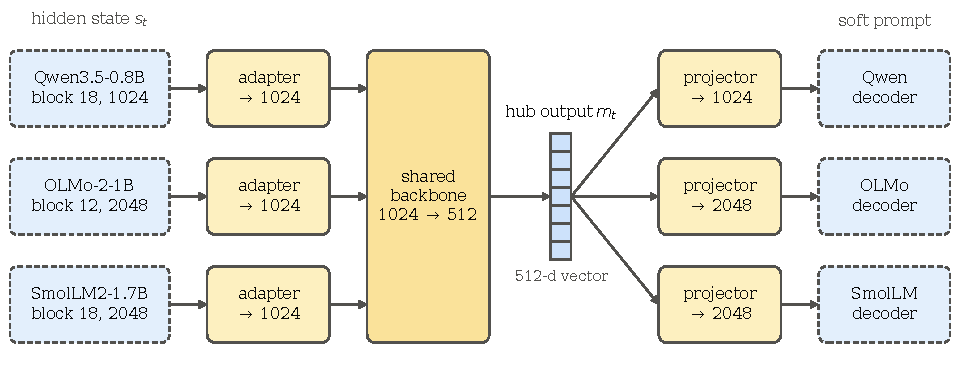
\includegraphics[width=\textwidth]{ch3/hub_architecture}
\caption{The translation hub maps each model's hidden states into one shared space, and every frozen model decodes from it.
Model-specific adapters and a shared backbone produce the 512-dimensional hub output; model-specific projectors map it into the input space of each frozen decoder.
Shaded boxes are trainable modules, dashed boxes are frozen models, and the column of cells is the hub output, a vector with no parameters of its own.}
\label{fig:hub:arch}
\end{figure}

\paragraph{Into the hub.} The source adapter of model $a$ maps its hidden state $s_t$ to a common width of \vf{1024}; a shared backbone then produces the hub output $m_t$ of \vf{512} dimensions:
\begin{equation}
m_t = W_h\, R_0\big(R_a(W_a s_t + b_a)\big) + b_h,
\qquad
R(z) = z + V_2\,\mathrm{SiLU}\big(V_1\,\mathrm{LN}(z) + c_1\big) + c_2 .
\label{eq:hub:map}
\end{equation}
Here $W_a$ is the linear layer of model $a$'s adapter, $R_a$ its residual block, $R_0$ the residual block of the shared backbone, and $W_h$ the shared linear layer from \vf{1024} to \vf{512}.
Each residual block $R$ applies layer normalization (LN) and a SiLU activation, widens to \vf{2048}, and returns to \vf{1024}. % src: src/v3/bridge.py (SourceAdapter, ResidualMLP); src/v6_2/bridge.py (H3BridgeBundle); configs/v6_3.yaml (architecture)

\paragraph{Out of the hub.} A hub output leaves the hub through a model-specific affine projector, which maps $m_t$ to the input width of a frozen language model, the decoder.
The projected vectors form a soft prompt with one row per source token.
The decoder generates the reconstructed prompt after its start token.

\paragraph{Models and directions.} The three models are Qwen3.5-0.8B, OLMo-2-1B, and SmolLM2-1.7B.
Each contributes hidden states from the block at three quarters of its depth: block \vf{18} of \vf{24} in Qwen (width \vf{1024}), block \vf{12} of \vf{16} in OLMo (width \vf{2048}), and block \vf{18} of \vf{24} in SmolLM (width \vf{2048}). % src: configs/v6_3.yaml (d3_block, width); configs/v3.yaml (blocks, depth_fractions)
% \todo{One sentence on why this depth, with its source.}
A direction pairs a source model with a decoder, e.g., Qwen $\to$ hub $\to$ OLMo.
Three models define nine directions: six cross-model directions and three self-reconstruction directions.
The cross-model directions test H1, because in them the decoder reconstructs from another model's states.
Only the adapters, the backbone, and the projectors are trainable; the three language models remain frozen as both sources and decoders.

\paragraph{Token-wise mapping.} The hub maps each token independently.
Equation~\ref{eq:hub:map} has no positional input and no attention across tokens, so each hub output depends on one source hidden state, although that state may already encode prompt context.
Chapter~\ref{ch:attack} depends on the token-wise design.

%% ------------------------------------------------------------------
\section{Training}\label{sec:hub:training}

Training is fully supervised: each prompt passes through all three frozen models, and every update includes all nine directions.
The objective combines a reconstruction loss with two alignment losses:
\begin{equation}
\mathcal{L} = \mathcal{L}_{\text{dec}} + 0.1\,\mathcal{L}_{\text{InfoNCE}} + 1.0\,\mathcal{L}_{\text{geom}} .
\label{eq:hub:loss}
\end{equation}
The decoding loss $\mathcal{L}_{\text{dec}}$ trains the hub to retain the input information that the frozen decoders need.
The contrastive loss $\mathcal{L}_{\text{InfoNCE}}$ encourages the three models to place the same text span at the same point of the hub.
The geometry loss $\mathcal{L}_{\text{geom}}$ encourages the hub to keep the similarities among spans that each model's hidden states already hold.

\paragraph{Decoding loss.} For each direction, the decoder receives the soft prompt, then its start token, then the ground-truth prompt tokens $x_1 \ldots x_T$, where $T$ is the prompt length in the decoder's own tokens.
Under teacher forcing the decoder makes $T+1$ predictions: the $T$ prompt tokens and then the end-of-sequence token.
The target is the prompt itself, not its continuation.
The loss of direction $d$, $\text{CE}_d$, averages cross-entropy over the $T+1$ predictions and then over prompts. % src: v6_3/plan.md section 4; src/v3/evaluate.py (teacher_forced_batch)
The decoding loss is a weighted mean over the nine directions:
\begin{equation}
\mathcal{L}_{\text{dec}} = \frac{1}{7}\Big(\sum_{d\,\in\,\text{cross}} \text{CE}_d + \frac{1}{3}\sum_{d\,\in\,\text{self}} \text{CE}_d\Big).
\label{eq:hub:dec}
\end{equation}
% src: src/v6_2/losses.py (weighted_direction_ce: (sum cross + 1/3 sum self)/7; h3_objective); configs/v6_3.yaml (loss)
Cross-model reconstruction thus accounts for $6/7$ of the decoding loss and self-reconstruction for $1/7$. % TODO(author): state why self-reconstruction is down-weighted; v6_2/plan.md fixes the weight without a reason

\paragraph{Token groups.} The two alignment losses compare models at corresponding positions of a prompt, yet the three tokenizers segment a prompt differently.
For each pair of models, the tokens are therefore collected into token groups: a group ends only at a character position where both tokenizers end a token (whitespace is ignored). % src: src/v3/alignment.py (connected components, a_weights, b_weights); src/v6_2/data.py (_pair_groups)
If one tokenizer splits \emph{unbelievable} into \emph{un \textbar{} believable} and the other into \emph{un \textbar{} believ \textbar{} able}, the word yields two groups: \emph{un}, with one token per model, and \emph{believable}, with one token under the first model and two under the second.
Each model contributes one vector per group: the mean of its token vectors, weighted by character coverage and normalized to unit length.

\paragraph{Contrastive loss.} For a model pair $(a,b)$, let $g^a_i$ and $g^b_i$ be the group vectors of group $i$, computed from the hub outputs of models $a$ and $b$.
The positive pair is $(g^a_i, g^b_i)$: one text span of one prompt, represented by two models.
The negatives are the vectors $g^b_j$ of groups from other prompts in the batch:
\begin{equation}
\ell^{\,a\to b}_i = -\log\frac{\exp(g^a_i\cdot g^b_i/\tau)}{\sum_{j\in\mathcal{N}_i}\exp(g^a_i\cdot g^b_j/\tau)},
\qquad \tau = 0.05 ,
\label{eq:hub:infonce}
\end{equation}
where $\mathcal{N}_i$ contains group $i$ and its negatives.
The loss is averaged over groups within each prompt, then over prompts, over the two orders of each pair, and over the three model pairs. % src: src/v3/losses.py (_symmetric_group_info_nce_encoded, _negative_mask_from_codes, _mean_within_query_codes, grouped_info_nce)

\paragraph{Geometry loss.} For model $a$ of a pair, let the rows of $X_a$ be the group vectors computed from its hidden states and the rows of $Y_a$ the group vectors computed from its hub outputs.
Each token vector is first centered on the model's mean hidden state or mean hub output.
The Gram matrix $\Gamma(A) = AA^{\top}$ of a matrix $A$ of group vectors contains the inner products between groups.
The distance $d(A,B)$ is the mean squared difference between the off-diagonal entries of $\Gamma(A)$ and $\Gamma(B)$.
The loss is
\begin{equation}
\mathcal{L}_{\text{geom}} = \tfrac{1}{2}\Big(\overline{d(X_a, Y_a)} + \overline{d(Y_a, Y_b)}\Big),
\label{eq:hub:geom}
\end{equation}
where the first bar denotes a mean over the two models of each pair and over the three pairs, and the second a mean over the three pairs.
The first term compares one model with itself: the similarities among its hub outputs should match those among its hidden states.
The second term compares two models: the similarities among the hub outputs of model $a$ should match those of model $b$ on the same groups. % src: src/v4/geometry.py; src/v6_2/train.py (_geometry_sides, compute_initial_statistics)

\paragraph{Schedule and checkpoint selection.} The hub is trained for \vf{2{,}500} AdamW updates of \vf{32} prompts each, drawn from \vf{40{,}000} training prompts, with one random seed.
The learning rate rises to $3\times10^{-4}$ over \vf{250} warmup updates and follows a cosine decay to zero; weight decay is \vf{0.01} on the linear weights, and gradients are clipped at norm \vf{1.0}. % src: configs/v6_3.yaml (training)
Teacher-forced Acc@1 selects the checkpoint.
Acc@1 is the fraction of prompt tokens that the decoder ranks first given the ground-truth prefix, averaged over the \vf{5{,}000} validation prompts and the six cross-model directions.
A checkpoint is scored every \vf{250} updates, and the earliest within \vf{0.002} of the best is retained: on Corpus A (Natural Questions queries), update \vf{2{,}250}, at Acc@1 \vf{0.954}. % src: results/v6_3/hpc-final/report.json (selected_step, cross_mean); src/v3/evaluate.py (content_accuracy_at1)

%% ------------------------------------------------------------------
\section{Evaluation}\label{sec:hub:eval}

\paragraph{Free-running decoding.} H1 is evaluated under free-running decoding, because under teacher forcing the ground-truth prefix carries information about the next token.
Each decoder conditions on the soft prompt and on its own generated prefix; greedy generation starts at the start token and stops at the end-of-sequence token or at the generation cap.
The cap is the length of the soft prompt plus \vf{32} tokens on the legal corpora. % TODO(author): state the cap on Corpus A

\paragraph{Metrics.} Two metrics compare the reconstruction with the source prompt.
Word-F1 is the harmonic mean of word precision and recall over word multisets, averaged over prompts.
Exact match is the fraction of reconstructions equal to their source prompt after Unicode and whitespace normalization.
Word-F1 ignores word order, so exact match is reported beside it as the order-sensitive metric.

\paragraph{Mismatched-prompt control.} A fluent decoder may score above zero without reading its soft prompt, because prompts of one corpus share common words.
The mismatched-prompt control measures that floor: the decoder receives the hub outputs of another prompt, and its output is scored against the original prompt.
Prompt $i$ receives the hub outputs of prompt $i+1$, and the last prompt those of the first. % src: src/v6_3/inversion.py (shuffled_indices: (i + 1) mod n); src/v8/projectors.py (wrong_partner: same rule)
A score above its control shows that the reconstruction depends on the prompt's own hub outputs.

\paragraph{Corpus A.} Corpus A contains query strings from Natural Questions, split into \vf{40{,}000} training, \vf{5{,}000} validation, and \vf{5{,}000} test prompts.
Near-duplicate questions never cross a split. % src: configs/v3.yaml (split_schema_version v2-stage2-textcluster-v1); src/v3/splits.py
The validation prompts average \vf{9} words and range from \vf{6} to \vf{19}. % src: configs/v3.yaml (n_train, n_val, n_test); word counts from the references in results/v6_3/hpc-final/inversion-records.jsonl (mean 9.08, median 9)
All scores in this chapter are computed on the validation split, which also selects the checkpoint, so no score is held out; the test split has not been evaluated.

\paragraph{Criteria for H1.} One score summarizes a hub: mean cross-model word-F1, the free-running word-F1 averaged over the six cross-model directions on the validation split.
A corpus fails H1 if that mean falls below \vf{0.90} or if the mismatched-prompt control on the same prompts reaches \vf{0.20}.
Both thresholds come from the evaluation plan of the legal hubs and were applied to Corpus A retrospectively. % src: v8_3/plan.md (0.90 and control below 0.20, readiness thresholds); no threshold precedes the Corpus A run

%% ------------------------------------------------------------------
\section{Results on Question Prompts}\label{sec:hub:results}\label{sec:hub:translation}

Cross-model reconstruction on Corpus A meets both criteria for H1.
On the \vf{5{,}000} validation prompts, cross-model word-F1 averages \vf{0.945}, against \vf{0.120} under the mismatched-prompt control; exact match averages \vf{0.71} and is zero under the control. % src: results/v6_3/hpc-final/inversion.json cross_mean (hub 0.9445, exact 0.7116; shuffled 0.1203, exact 0.0)
The gap above the mismatched-prompt control shows that the reconstruction depends on the prompt's own hub outputs.

\begin{figure}[ht]
\centering
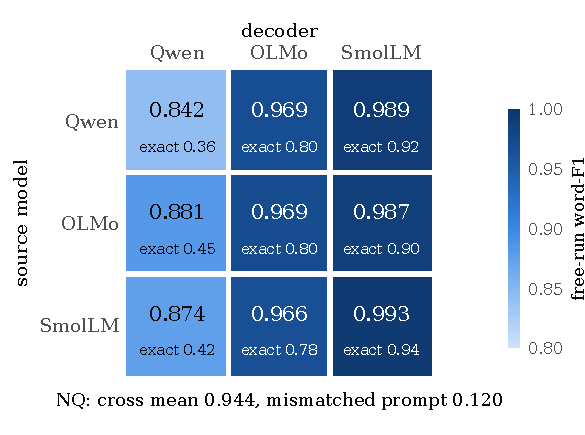
\includegraphics[width=0.62\textwidth]{ch3/direction_recovery_nq}
\caption{The OLMo and SmolLM decoders reconstruct every source above 0.96 word-F1; the Qwen decoder reaches 0.84 to 0.88.
Free-running word-F1, with exact match below, by source model (rows) and decoder (columns) on the \vf{5{,}000} Corpus A validation prompts; diagonal cells are self-reconstruction.
The mismatched-prompt control scores \vf{0.120} to \vf{0.121} in every direction.
One hub seed.}
\label{fig:hub:directions}
\end{figure}

The mean hides one weaker decoder (Figure~\ref{fig:hub:directions}).
The four cross-model directions into OLMo and SmolLM score \vf{0.966} to \vf{0.990}; the two into Qwen score \vf{0.881} and \vf{0.874}, below the \vf{0.90} required of the mean. % src: results/v6_3/hpc-final/inversion.json directions

Table~\ref{tab:hub:examples} shows reconstructions from OLMo $\to$ Qwen. % src: results/v6_3/hpc-final/inversion-records.jsonl, olmo->qwen hub arm

\begin{table}[H]
\caption{At an intermediate score one word changes; at a low score the names are lost.
Reconstructions from OLMo $\to$ Qwen on Corpus A validation prompts, selected at high, intermediate, and low word-F1; the final row is generated under the mismatched-prompt control and scored against the original prompt.
Decoded words that match the true prompt are green; the others are orange and bold.}
\label{tab:hub:examples}
\centering
\small
\begin{tabular}{@{}p{0.27\textwidth}p{0.68\textwidth}@{}}
\toprule
True prompt & who played uncle in only fools and horses \\
Decoded, word-F1 \vf{1.00} & \hit{who played uncle in only fools and horses} \\
\midrule
True prompt & who has sang most songs in the world \\
Decoded, word-F1 \vf{0.88} & \hit{who has} \miss{sung} \hit{most songs in the world} \\
\midrule
True prompt & is floral park in queens or long island \\
Decoded, word-F1 \vf{0.50} & \hit{is} \miss{flower} \hit{park in} \miss{king} \hit{or} \miss{queen parks} \\
\midrule
True prompt & who played uncle in only fools and horses \\
Mismatched prompt, word-F1 \vf{0.25} & \hit{who} \miss{plays the girl jinx} \hit{in} \miss{suicide squad} \\
\bottomrule
\end{tabular}
\end{table}

%% ------------------------------------------------------------------
\section{Results on Legal Text}\label{sec:hub:legal}

Two legal corpora test H1 on text that differs from question prompts in vocabulary and in length.
A separate hub is trained per corpus, with the architecture and objective of Sections~\ref{sec:hub:design} and~\ref{sec:hub:training}.

\paragraph{Corpora.} The corpus legal128w cuts one contiguous window per legal document, with the start word drawn uniformly over the document; its validation prompts average \vf{61} words. % src: references in results/legal128w/v6_3/inversion-records.jsonl, first 5,000 records (mean 61.2, range 8 to 90)
The corpus legal10w cuts ten consecutive words from the same source documents, from a start word drawn uniformly over the document. % src: documents/glossary.md (window corpus, piece corpus)
Each corpus has \vf{40{,}000} training and \vf{5{,}000} validation prompts. % src: configs/v6_3_legal{128w,10w}.yaml (n_train, n_validation)

\paragraph{Results.} Both legal hubs meet both criteria for H1 (Table~\ref{tab:hub:legal}).
Mean cross-model word-F1 is \vf{0.977} on each corpus, against mismatched-prompt controls of \vf{0.152} on legal128w and \vf{0.071} on legal10w. % src: results/legal{128w,10w}/v6_3/inversion.json cross_mean (hub 0.9769, 0.9767; shuffled 0.1519, 0.0706)
Every cross-model direction exceeds \vf{0.90}; the lowest is Qwen $\to$ OLMo on legal128w, at \vf{0.955} (Figure~\ref{fig:hub:legal-directions}). % src: same files, directions (cross minima 0.9552, 0.9670)
The lower scores into Qwen on Corpus A do not recur: the cross-model directions into Qwen score \vf{0.975} to \vf{0.986}. % src: same files, olmo->qwen and smollm->qwen (0.9842, 0.9784; 0.9858, 0.9752)
Exact match is lower on the long prompts of legal128w, at \vf{0.58}, than on the ten-word prompts of legal10w, at \vf{0.83}; the comparison does not isolate length from content.

\begin{table}[H]
\caption{Each legal hub exceeds a mean cross-model word-F1 of \vf{0.90} with a control below \vf{0.20}.
Free-running word-F1 and exact match averaged over the six cross-model directions on the \vf{5{,}000} validation prompts of each corpus, one hub seed per corpus; each control is evaluated on the same prompts and directions as its score.}
\label{tab:hub:legal}
\centering
\begin{tabular}{lccc}
\toprule
Corpus & Word-F1 & Exact match & Control word-F1 \\
\midrule
legal128w & \vf{0.977} & \vf{0.58} & \vf{0.152} \\ % src: results/legal128w/v6_3/inversion.json cross_mean (0.9769, 0.5814, 0.1519)
legal10w & \vf{0.977} & \vf{0.83} & \vf{0.071} \\ % src: results/legal10w/v6_3/inversion.json cross_mean (0.9767, 0.8291, 0.0706)
\bottomrule
\end{tabular}
\end{table}

\begin{figure}[ht]
\centering
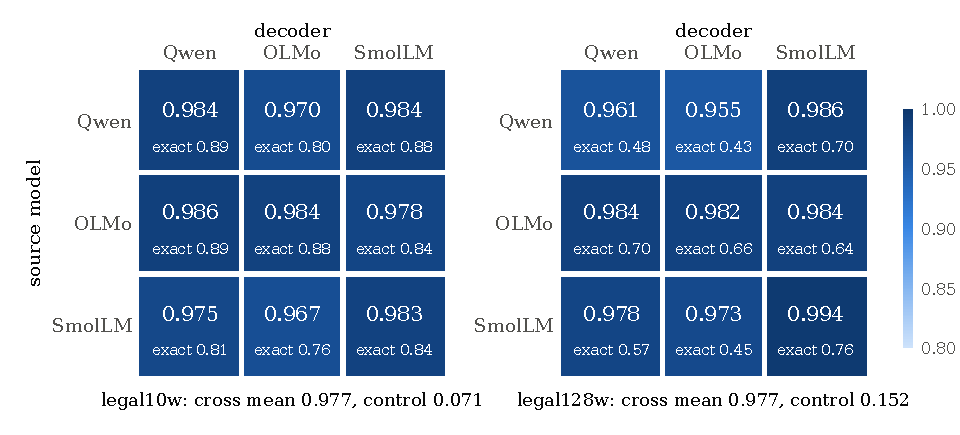
\includegraphics[width=\textwidth]{ch3/direction_recovery_legal}
\caption{Every direction of the two legal hubs reaches a word-F1 of at least 0.95.
Free-running word-F1, with exact match below, by source model (rows) and decoder (columns) on the \vf{5{,}000} validation prompts of each legal corpus; diagonal cells are self-reconstruction.
One hub seed per corpus.}
\label{fig:hub:legal-directions}
\end{figure}

%% ------------------------------------------------------------------
\section{Discussion}\label{sec:hub:discussion}

The results support H1 on three corpora.
Each of three frozen models reconstructs a prompt from the hidden states of the other two, at a mean word-F1 of \vf{0.945} on Corpus A and \vf{0.977} on the two legal corpora, with every mismatched-prompt control below \vf{0.20}.
%% BIG CHANGE: states what the result means for the hypothesis that motivates the chapter (shortened 2026-11-15).
The three models were trained separately, yet one shared space preserves the prompt from each, which is what the Platonic Representation Hypothesis predicts.

%% BIG CHANGE: limitations restored from the commented-out list of draft_v3 and stated once, here (shortened 2026-11-15).
Three limits bound the claim.
The hub is trained with full supervision, so the result shows that a shared space can be learned for these models, not that their hidden states align without training.
Each corpus has its own hub, one seed, and scores on the validation split that selected the checkpoint.
No pairwise baseline is reported, so no advantage of a hub over model-to-model maps is established.

The first limit sets the question of Chapter~\ref{ch:attack}: whether a target model outside hub training reaches the same space through one affine map fitted on a small leak.
